%\documentclass[0-main.tex]{subfiles}
%\begin{document}

\section{Experiments}\label{sec:exp}
We evaluate \hirl on two standard RL benchmarks and in deformable cutting and tensioning on the da Vinci surgical robot.

\begin{figure}[t]
\centering
 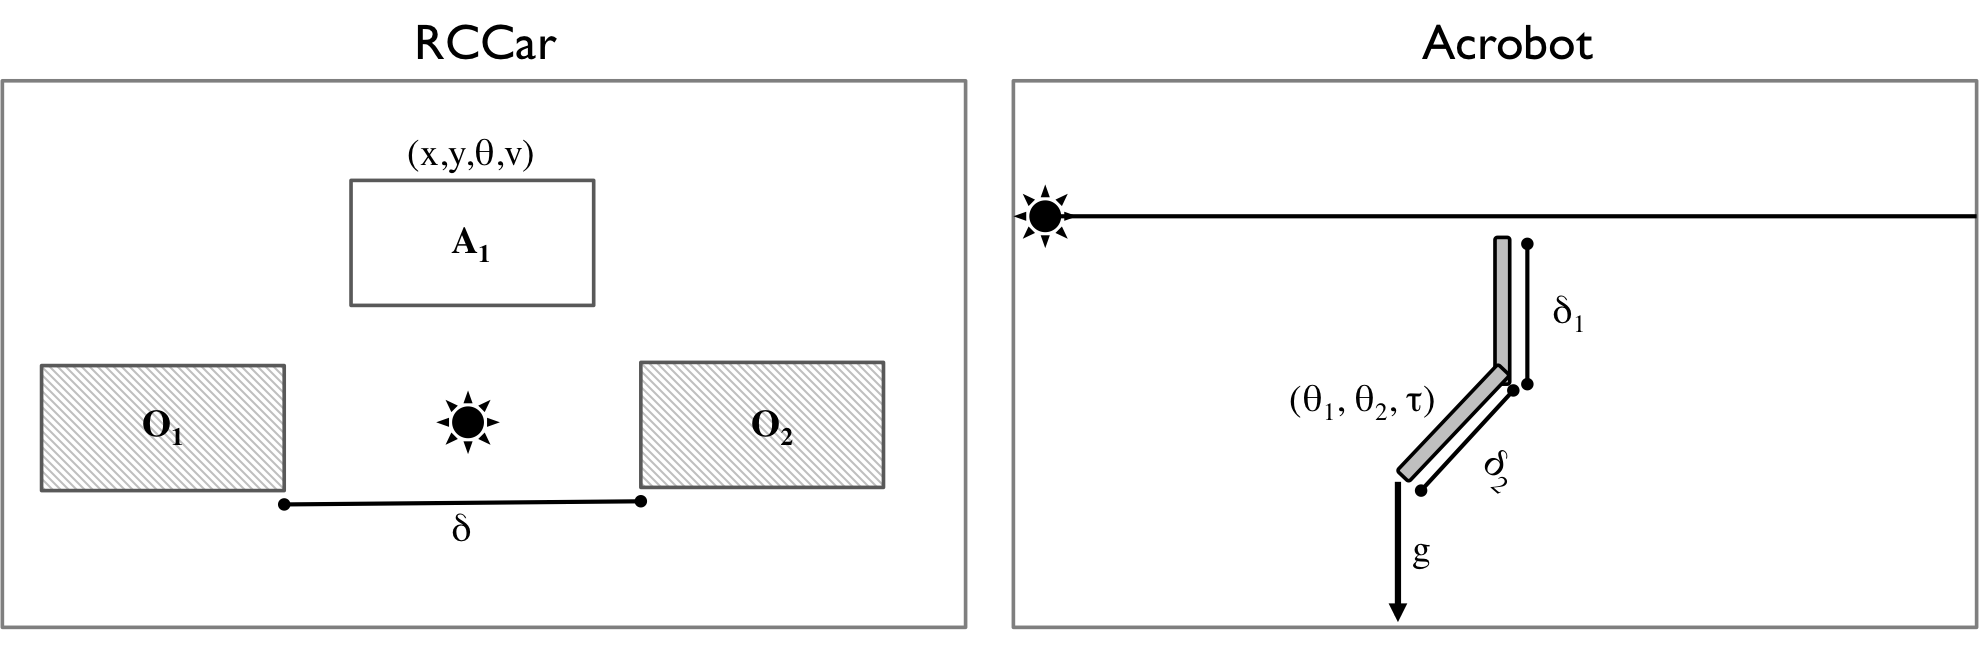
\includegraphics[width=\columnwidth]{figures/domains.png}
 \caption{(A) Simulated control task with a car with noisy non-holonomic dynamics. The car ($A_1$) is controlled by accelerating and turning in discrete increments. The task is to park the car between two obstacles. \label{domains}}
\end{figure}

\begin{figure}[t]
\centering
 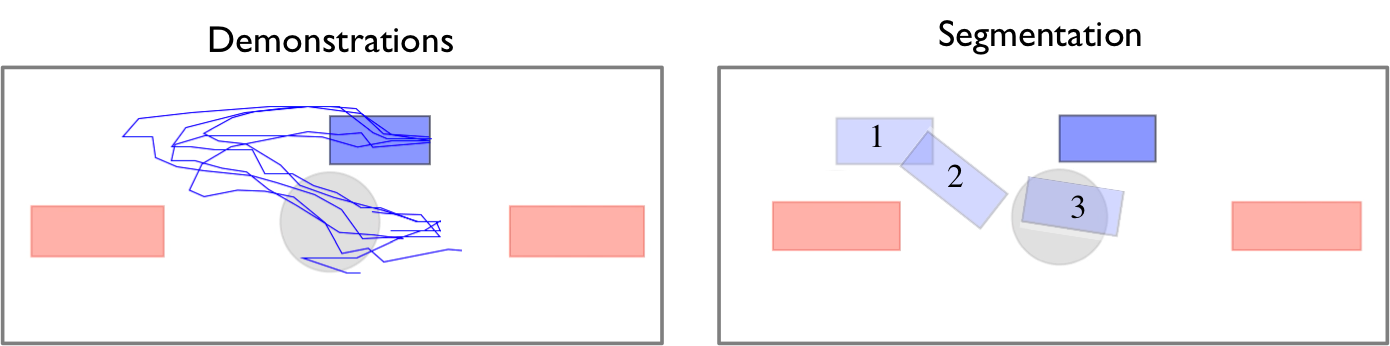
\includegraphics[width=\columnwidth]{exp/rc-car-segmentation.png}
 \caption{(Left) the 5 demonstration trajectories for the parallel parking task, and (Right) the sub-goals learned by \hirl. There are two intermediate goals corresponding to positioning the car and orienting the car correctly before reversing. \label{exp:rcsegmentation}}
\end{figure}

\subsection{Fully Observed Parallel Parking}\label{exp:pp}
We constructed a parallel parking scenario for a robot car with non-holonomic dynamics and two obstacles (Figure \ref{domains}a). 
The car can accelerate or decelerate in discrete $\pm 0.1$ meters per second increments (and reverse), and change its heading by $5^\circ$ degree increments.
The car's speed ($\|\dot{x}\|+\|\dot{y}\|$) and heading ($\theta$) are inputs to a bicycle steering model which computes the next state.
The car observe its x position, y position, orientation, and speed in a global coordinate frame.
The robot's dynamics are noisy and with probability 0.1 will randomly add or subtract $2.5^\circ$ degrees to the steering angle.
If the robot parks between the obstacles, i.e., 0 speed within a $15^\circ$ tolerance and a positional tolerance of $5$ meters, the task is a success and the robot receives a reward of $1$. 
If the robot collides with one of the obstacle or does not park in 200 timesteps the episode ends with a reward of $0$.

We call this domain Parallel Parking with Full Observation (PP-FO). We consider the following approaches:

\vspace{0.25em}\noindent \textbf{RL (Q-Learning): } The baseline approach is modeling the entire problem as an MDP with the sparse delayed reward. We apply Q-Learning to learn a policy for this problem with a radial basis function representation for the Q function with number of bases and bandwidth $k=5, \sigma=0.1$ respectively. The radial basis function hyper-parameters were tuned manually to achieve the fastest convergence in the experimental task. 

\vspace{0.25em}\noindent \textbf{Behavioral Cloning (SVM): } We generated $N$ demonstrations using an RRT motion planner (assuming deterministic dynamics). The next baseline is to directly learn a policy from the generated plans using behavioral cloning. We use a L1 hinge-loss SVM with L2 regularization $\alpha=5e-3$ to predict the action from the state. The hyper-parameters were tuned manually using cross-validation by holding out trajectories.

\vspace{0.25em}\noindent \textbf{Single-Step IRL (MaxEnt-IRL): } We generated $N$ demonstrations using an RRT motion planner (assuming deterministic dynamics). We use the collected demonstrations and infer a quadratic reward function using MaxEnt-IRL (both using estimated dynamics and ground truth dynamics). The learned reward function is optimized using Q-learning with a radial basis function representation with the same hyper-parameters as the RL approach. 

\vspace{0.25em}\noindent \textbf{\hirl: } Finally, we apply \hirl to the $N$ demonstrations, learn segmentation, and quadratic rewards (Figure~\ref{exp:rcsegmentation}).
We apply \hirl with a DP-GMM based segmentation step with no kernel transformation (as described in Section \ref{segm}).
For the local IRL approach, we consider three approaches: MaxEnt with ground truth dynamics, MaxEnt with locally estimated dynamics, Model-Free. 
The learned reward functions and transition regions are used in the policy learning phase with Q-learning with a radial basis function representation with the same hyper-parameters as the RL approach.

\vspace{0.5em}

\subsubsection{Fixed Demonstrations, Vary Rollouts}
In the first experiment, we fix number of initial demonstrations $N=5$, and vary the number of rollouts.

\subsubsection{Fixed Rollouts, Vary Demonstrations}
Next, we fix the number of rollouts to $1250$, and vary the number of demonstration trajectories each approach observes.
In the fully observed problem, compared to MaxEnt-IRL, the model-based \hirl converges to a policy with a 60\% success rate with about 3x fewer time-steps.
The gains for the model-free version are more modest with a 50\% reduction.
The supervised policy learning approach achieves a success rate of 47\% and the baseline RL approach achieves a success rate of 36\% after 250000 time-steps.

The baseline Q-Learning approach directly tries to learn a sequence of actions to minimize the quadratic cost around the target state. 
This leads to a lot of exploration since the robot must first make ``negative'' progress (pulling forward). 
\hirl improves convergence since it structures the exploration through the segmentation.
The local reward functions are better shaped to guide the car towards its short term goal.
This focuses the exploration on solving the short term problem first.
MaxEnt-IRL mitigates some of the problems since it rewards states based on their estimated cost-to-go, but as the time-horizon increases the estimates of this become nosier--leading to worse performance (see technical report for a characterization~\cite{krishnan2016hirl}).


\subsubsection{Vary Task Parameters}
Finally, we explore how well the constructed rewards transfer if the dynamics are perturbed in the fully observed setting.
We expect MaxEnt-IRL to transfer well because it learns a delayed reward, which tends to encode success conditions and not task-specific details.
After constructing the rewards, we randomly perturbed the system dynamics by introducing a bias towards turning left.
We find that the model-based \hirl technique transfers to this domain comparably to MaxEnt-IRL until the task is so different that the sub-goals learned with \hirl are no longer informative.
The model-free \hirl algorithm converges more slowly; requiring 20\% more time-steps to converge to the same success rate. 



\subsection{Partially Observed Parallel Parking}
Next, we made the  Parallel Parking domain a little harder. We hid the velocity state from the robot, so the robot only sees $(x,y,\theta)$. As before, if the robot collides with one of the obstacle or does not park in 200 timesteps the episode ends.
We call this domain Parallel Parking with Partial Observation (PP-PO).

As before, we generated 5 demonstrations using an RRT motion planner (assuming deterministic dynamics) and applied \hirl to learn the segments.
Figure \ref{exp:rcsegmentation} illustrates the demonstrations and the learned segments. 


In the partial observation problem (PP-PO), there is no longer a stationary policy that can achieve the reward.
The techniques that model this problem with a single MDP all fail to converge.
The learned segments in \hirl help disambiguate dependence on history.
After 250000 time-steps, the policy learned with model-based \hirl has a 70\% success rate in comparison to a <10\% success rate for the baseline RL, MaxEnt-IRL, and 0\% for the SVM.









\begin{figure}[t]
\centering
 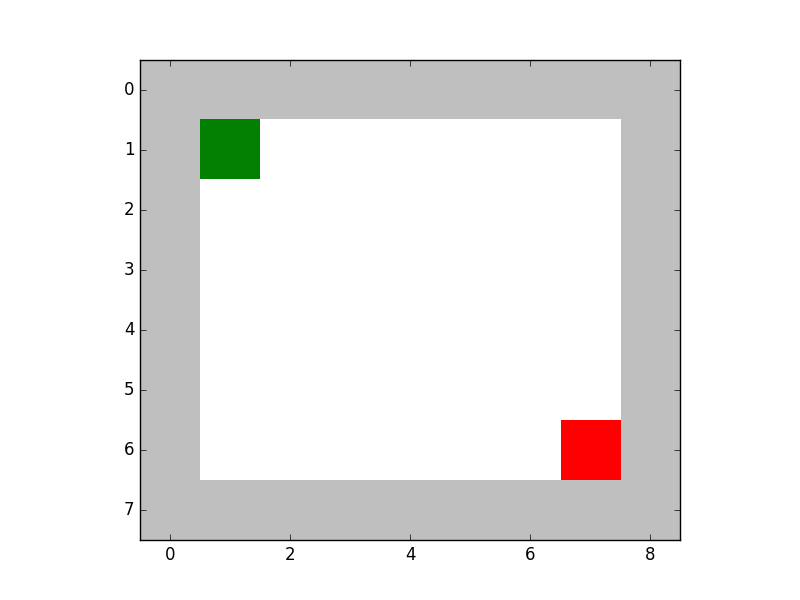
\includegraphics[width=0.32\columnwidth]{concept/swirl1-rewards.png}
  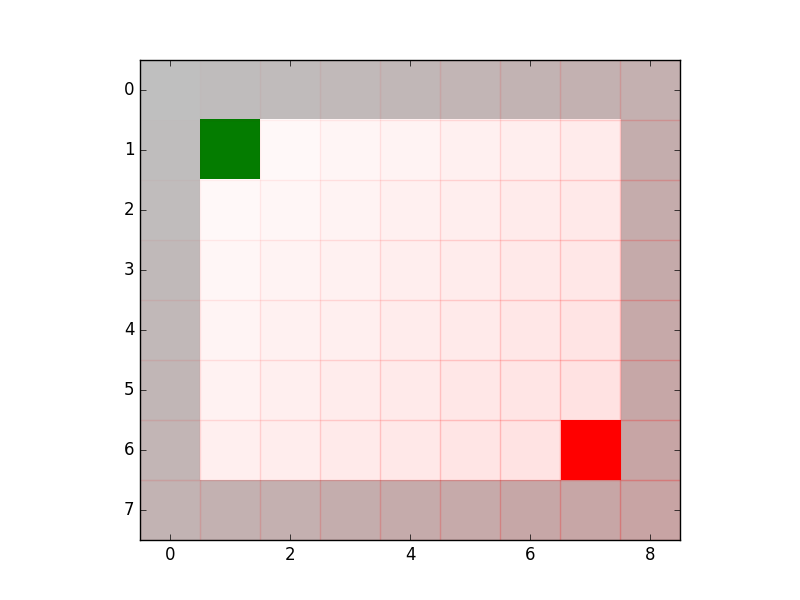
\includegraphics[width=0.32\columnwidth]{concept/swirl1-linear.png}
   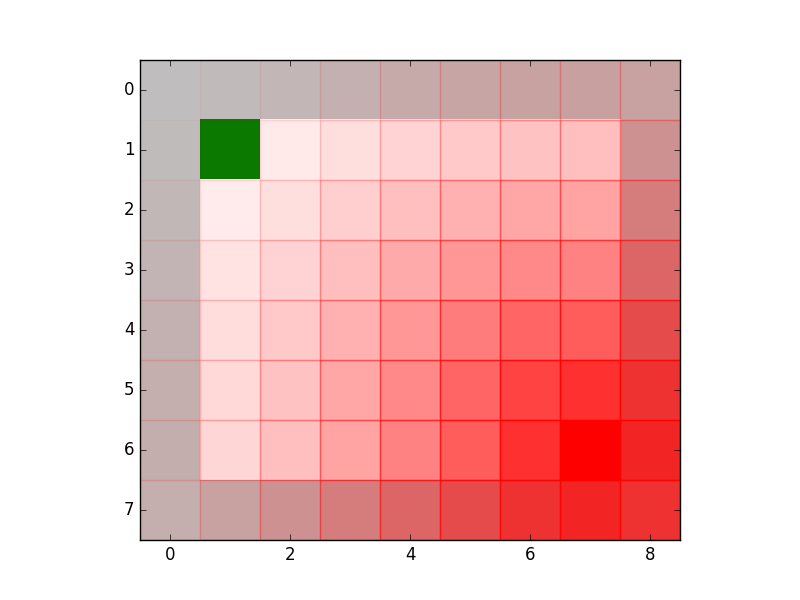
\includegraphics[width=0.32\columnwidth]{concept/swirl1-quadratic.png}
 \caption{This plot illustrates a conceptual GridWorld task. The green square denotes the starting position and the red denotes the target. The first plot shows the basic task, the second plot shows the reward learned with IRL from 5 demonstrations with a linear reward parametrization, and the second plot shows the reward learned with a quadratic parametrization. \label{concept:1}}
\end{figure}

\subsection{Conceptual Example: Discrete Planning}
We start with a GridWorld example to illustrate the structure of tasks amenable to segmentation. 

\vspace{0.5em} \noindent \textbf{Motivating Experiments: } Before we discuss segmentation, the first hypothesis that we have to evaluate is whether IRL on its own can improve the convergence of RL. This hypothesis is not unreasonable since some problem have a naturally sparse reward function (e.g., 1 if a goal state is reached, 0 else where), and IRL would approximate this reward with a smoother quadratic function. So consider an 16 x 16 GridWorld with a start position in one corner and a goal in another corner (Figure \ref{concept:1}a). 
The agent can move left, right, up, and down, and with a 30\% probability the action results in a random motion.
We sampled 5 demonstrations with a value iteration supervisor and applied IRL with linear and quadratic rewards. These results are visualized in (Figure \ref{concept:1}b-c).
These plots illustrate how IRL can be used to shape a reward function, by changing the reward parametrization. Even though the underlying reward function is a sparse 1/0 reward,  MaxEnt fits a linear or a quadratic reward function, which is smoother. These smoother reward functions can help guide the agent to the goal.

\begin{figure}[t]
\centering
 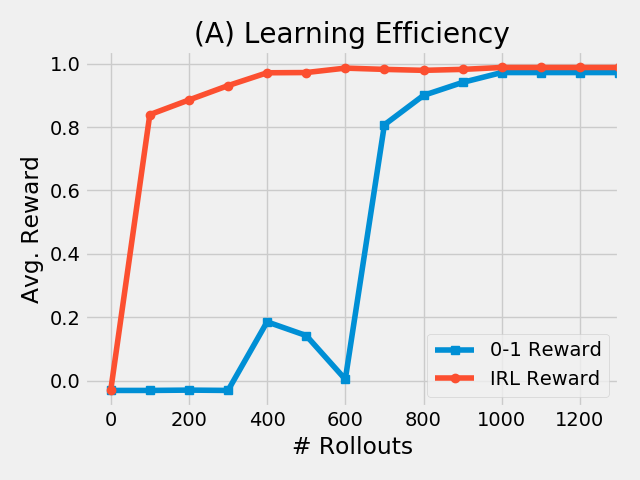
\includegraphics[width=0.48\columnwidth]{concept/1.png}
  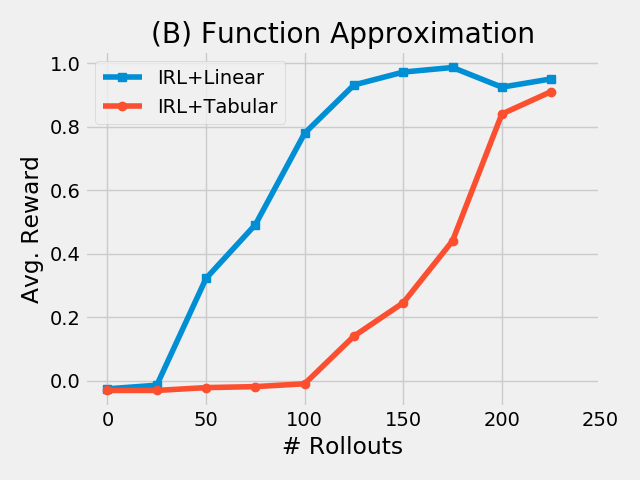
\includegraphics[width=0.48\columnwidth]{concept/2.png}
 \caption{(A) Tabular Q-Learning converges nearly 8x faster when the reward is quadratically shaped by IRL. (B) These benefits are even more pronounced when the Q function is approximated by a linear regression model. \label{concept:2}}
\end{figure}

If we were to compare the convergence of RL on the 1/0 reward and the quadratic reward, we find vastly different convergence properties.
We use a tabular Q-Learning agent with an $\epsilon$-greedy exploration policy ($\epsilon=0.1$).
Q-Learning on the quadratic reward converges in nearly 8x fewer steps than the 1/0 reward (Figure \ref{concept:2}a).
This is because the Q-Learning agent with the shaped reward function observes a reward earlier than the 0/1 agent, and thus, it is able to make progress towards the goal earlier in the learning process.
Combining function approximation with Q-Learning allows it to generalize to nearby unseen states.
The effects are even more pronounced since now once the agent observes the ``right direction'' to travel due to the shaped reward it is able to quickly make progress (Figure \ref{concept:2}b).
In the following experiments, we will use the term \textsf{IRL} to refer to the combined IRL+RL policy inference procedure.

\begin{figure}[t]
\centering
 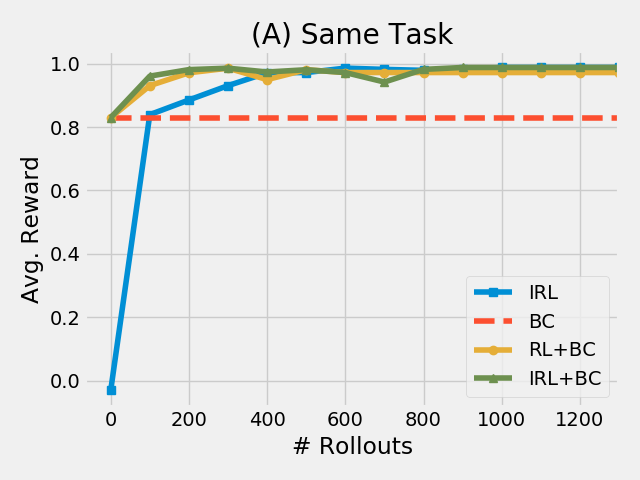
\includegraphics[width=0.48\columnwidth]{concept/3.png}
  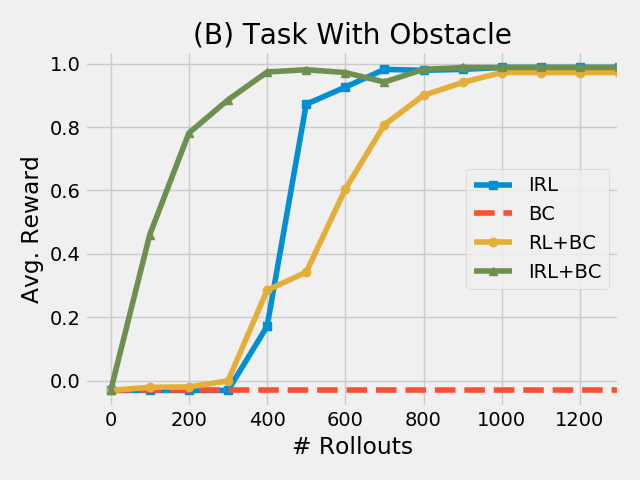
\includegraphics[width=0.48\columnwidth]{concept/4.png}
 \caption{(A) Given 5 expert demonstrations, Behavioral Cloning with a Random Forest classifier achieves a high reward on the same task. This can be used to initialize the Q-Learning agents. On the same task there is a marginal benefit to IRL. (B) We perturb the task after collecting 5 demonstrations by adding an obstacle blocking the shortest path, and find that the IRL agent is the most effective.  \label{concept:3}}
\end{figure}

One could hand-craft such reward functions, but one advantage of IRL is that it learns such functions from demonstration data. Admittedly, the previous comparison with RL is not completely fair. The RL algorithm with the 1/0 reward does not use the demonstration data. In principle, one could train a policy with Behavioral Cloning and use that to initialize the RL agent. Given the same 5 initial demonstrations, we train a random forest classifier.
When we apply this policy to the same task instance where the demonstrations were collected, the behavioral cloning policy does very well (Figure \ref{concept:3}a).
This can be used as an initialization to the Q-learning agent, which can further improve the policy.
On the same task instance, there is a marginal benefit to using IRL to shape the reward--as the behavioral cloning policy already gets the agent very close to the goal in most cases.

However, suppose that demonstration domain slightly differs from the execution domain. We simulate this by adding a 4x4 obstacle in the center of the GridWorld map.
Now, the learned behavioral cloning policy is not effective on the new domain (Figure \ref{concept:3}b).
However, the reward function learned with IRL transfers more robustly.
Furthermore, combining the IRL with a BC initialization improves performance over RL by 6x.
These results motivate us to consider how to use demonstrations to improve the convergence of RL.
In more complex tasks, a quadratic approximation of the reward may not suffice.
Hence, we consider how to segment the task into sub-tasks that can be approximated with a quadratic reward.


\begin{figure}[t]
\centering
 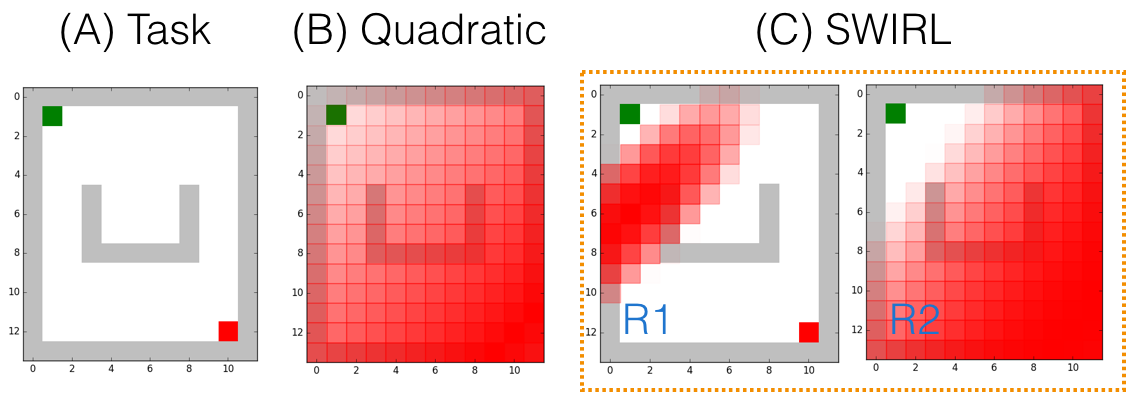
\includegraphics[width=\columnwidth]{concept/swirl-rewards.png}
 \caption{(A) A GridWorld domain with an obstacle, (B) Visualization of the reward function if we apply IRL to 5 demonstrations and fit a quadratic reward. The quadratic reward can encourage the agent to get ``stuck'' in the obstacle if it is too greedy, (C) Segmented quadratic reward function learned with \hirl. The function has two components first guiding the agent to the passage on the left, and then guiding to the goal.  \label{concept:4}}
\end{figure}

\begin{figure}[t]
\centering
 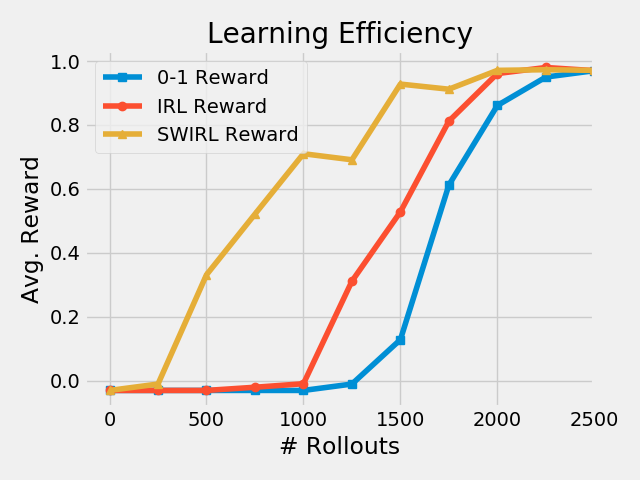
\includegraphics[width=0.6\columnwidth]{concept/2-1.png}
 \caption{\hirl converges faster than a single quadratic reward or the 1-0 reward. \label{concept:5}}
\end{figure}


\vspace{0.5em} \noindent \textbf{Hypothesis 0. IRL Can Benefit From Segmentation: } Now, we make the domain above slightly more complicated. We add an obstacle in such a way that the straight-line path is no longer optimal (Figure \ref{concept:4}a). As before, we sample 5 demonstrations from a value iteration supervisor.
Qualitatively, the quadratic reward learned from IRL is misleading as it can guide an overly greedy agent into the obstacle(Figure \ref{concept:4}b). 
\hirl learns a two-segment reward, where first it guides the agent to a point in the left passage and then a reward around the goal (Figure \ref{concept:4}c).
The number of segments was determined by a Dirichlet process prior as described in the text.

To evaluate \hirl quantitatively, we use a tabular Q-learning agent to learn a policy using these rewards.
To control for initialization effects, the agents were initialized randomly (unlike the previous experiment) and used an $\epsilon=0.1$ exploration policy.
This results in a significant improvement in convergence as seen in Figure \label{concept:5}.

\begin{figure}[t]
\centering
 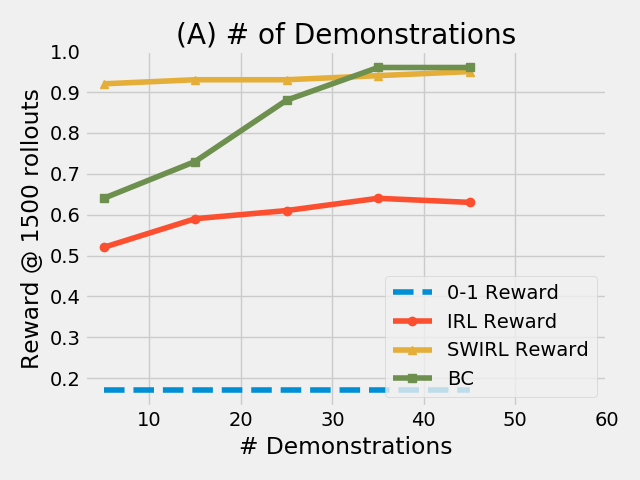
\includegraphics[width=0.48\columnwidth]{concept/3-1.png}
  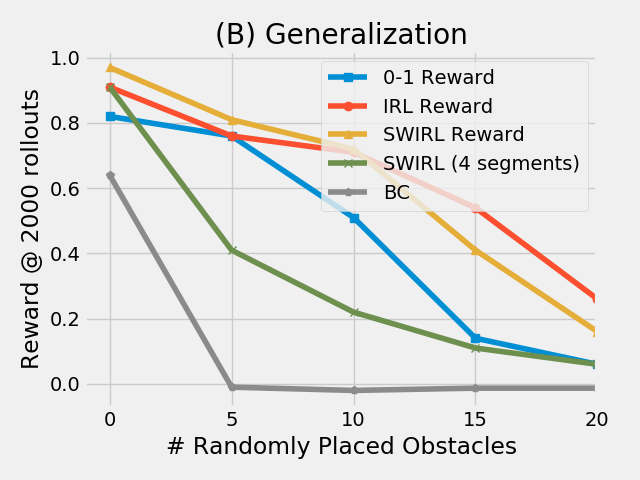
\includegraphics[width=0.48\columnwidth]{concept/3-2.png}
 \caption{(A) We measure the sensitivity to the number of initial demonstrations, (B) We perturb the execution environment by adding random obstacles. \label{concept:6}}
\end{figure}

\vspace{0.5em} \noindent \textbf{Parameter Sensitivity: } Finally, we use the previous GridWorld environment to illustrate the sensitivity to different parameters. In Figure \ref{concept:6}a, we vary the number of initial demonstrations provided to IRL and Behavioral Cloning and measure the performance after 1500 rollouts.
IRL is not as sensitive to the number of demonstrations as BC.
This is because the reward function that IRL is estimating is much simpler than policy function.
Next, we evaluate each of the algorithms on their ability to generalize to different task instances.
We perturb the execution environment by randomly adding single grid point obstacles.
We average the results over 50 such random perturbations (Figure \ref{concept:6}b).

Not surprisingly, we find that IRL is the most robust.
\hirl is relatively robust but is slightly worse than IRL for a large number of random obstacles.
We wanted to understand why \hirl was less robust than standard IRL, so we manually set the number of segments in \hirl to $4$.
The performance of \hirl with 4 segments is much worse.
This is because obstacles can ``invalidate'' segments.
This suggests an interesting tradeoff where more segments can serve to more precisely guide the agent towards the goal, but less segments lead to improved generalization.

\subsection{Simulated Control Domains}
Next, we describe \hirl on simulated control domains. These illustrate examples with continuous state-spaces.







\begin{figure*}[t]
\centering
 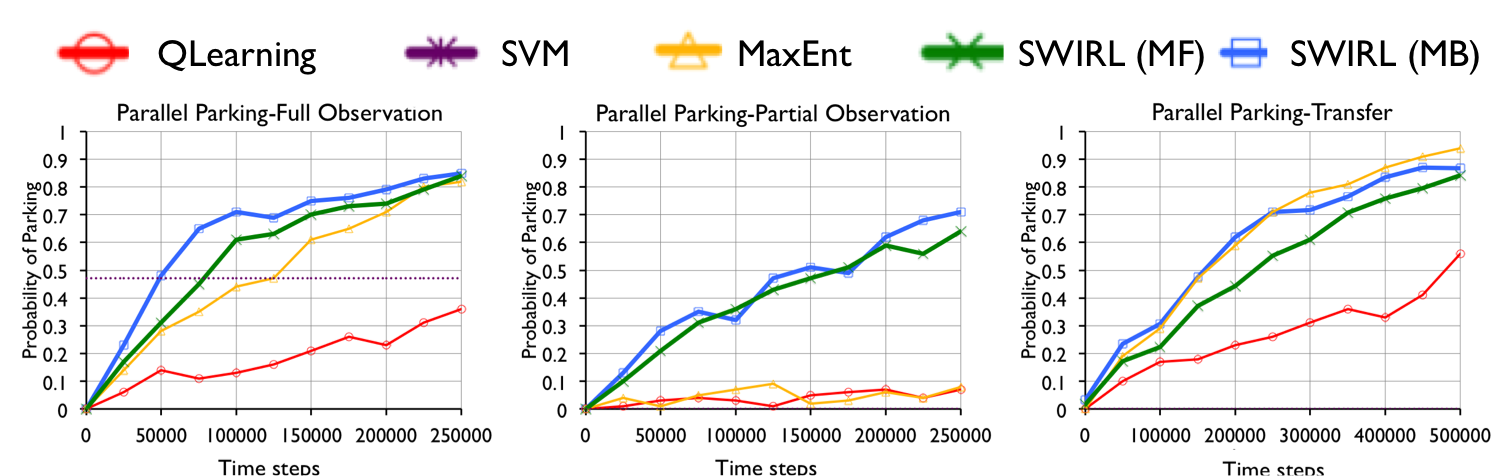
\includegraphics[width=0.8\textwidth]{exp/rc-convergence-1.png}
 \caption{Performance on a parallel parking task with noisy dynamics with full state observations (position, orientation, and velocity), partial observation (only position and orientation), and transfer (randomly permuting the action space).
 Success is measured in terms of the probability that the car successfully parked, and (M) denotes whether the approach used the dynamics model.
 In the fully observed case, both the model-based and model-free \hirl algorithms converge faster than MaxEnt-IRL and quickly outperforms the SVM.
 In the partially observed case, MaxEnt-IRL, Q-Learning, and the SVM fail--while \hirl succeeds.
 Both techniques also demonstrate comparable transferability to MaxEnt-IRL when the domain's dynamics are perturbed.
\label{exp:rcsegmentation-res}}
\end{figure*}



\begin{figure*}[t]
\centering
 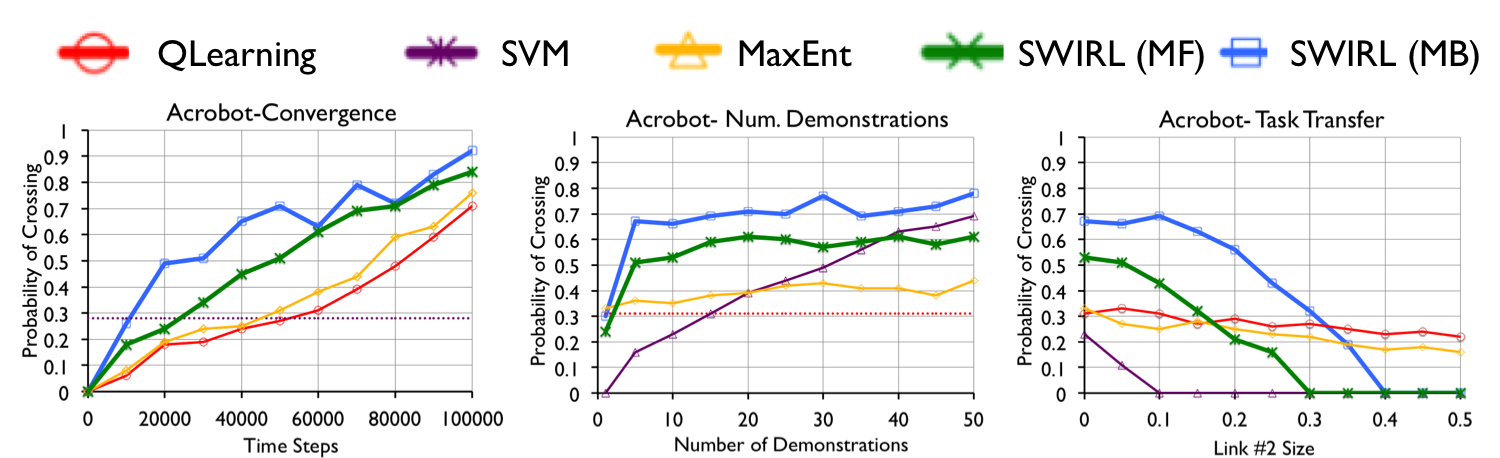
\includegraphics[width=0.8\textwidth]{exp/acr-convergence-1.png}
 \caption{Acrobot: We measured the performance of rewards constructed with \hirl and the alternatives. We find that \hirl (model-based and model-free) converges faster than MaxEnt-IRL, Q-Learning, and the SVM.
 Furthermore, \hirl requires less demonstrations, which we measure by comparing the performance of the alternatives after a fixed 50000 time-steps and with varied input demonstrations. 
 We also vary the task parameters by changing the size of the second link of the pendulum and find that the learned rewards are robust to this variation (as before comparing the performance of the alternatives after a fixed 50000 time steps). MaxEnt-IRL shows improved transfer performance since once the task has changed enough the segments learned during the demonstrations may not be informative and may even hurt performance if they are misleading. 
 \label{exp:acsegmentation-res2}}
\end{figure*}

\begin{figure}[t]
\centering
    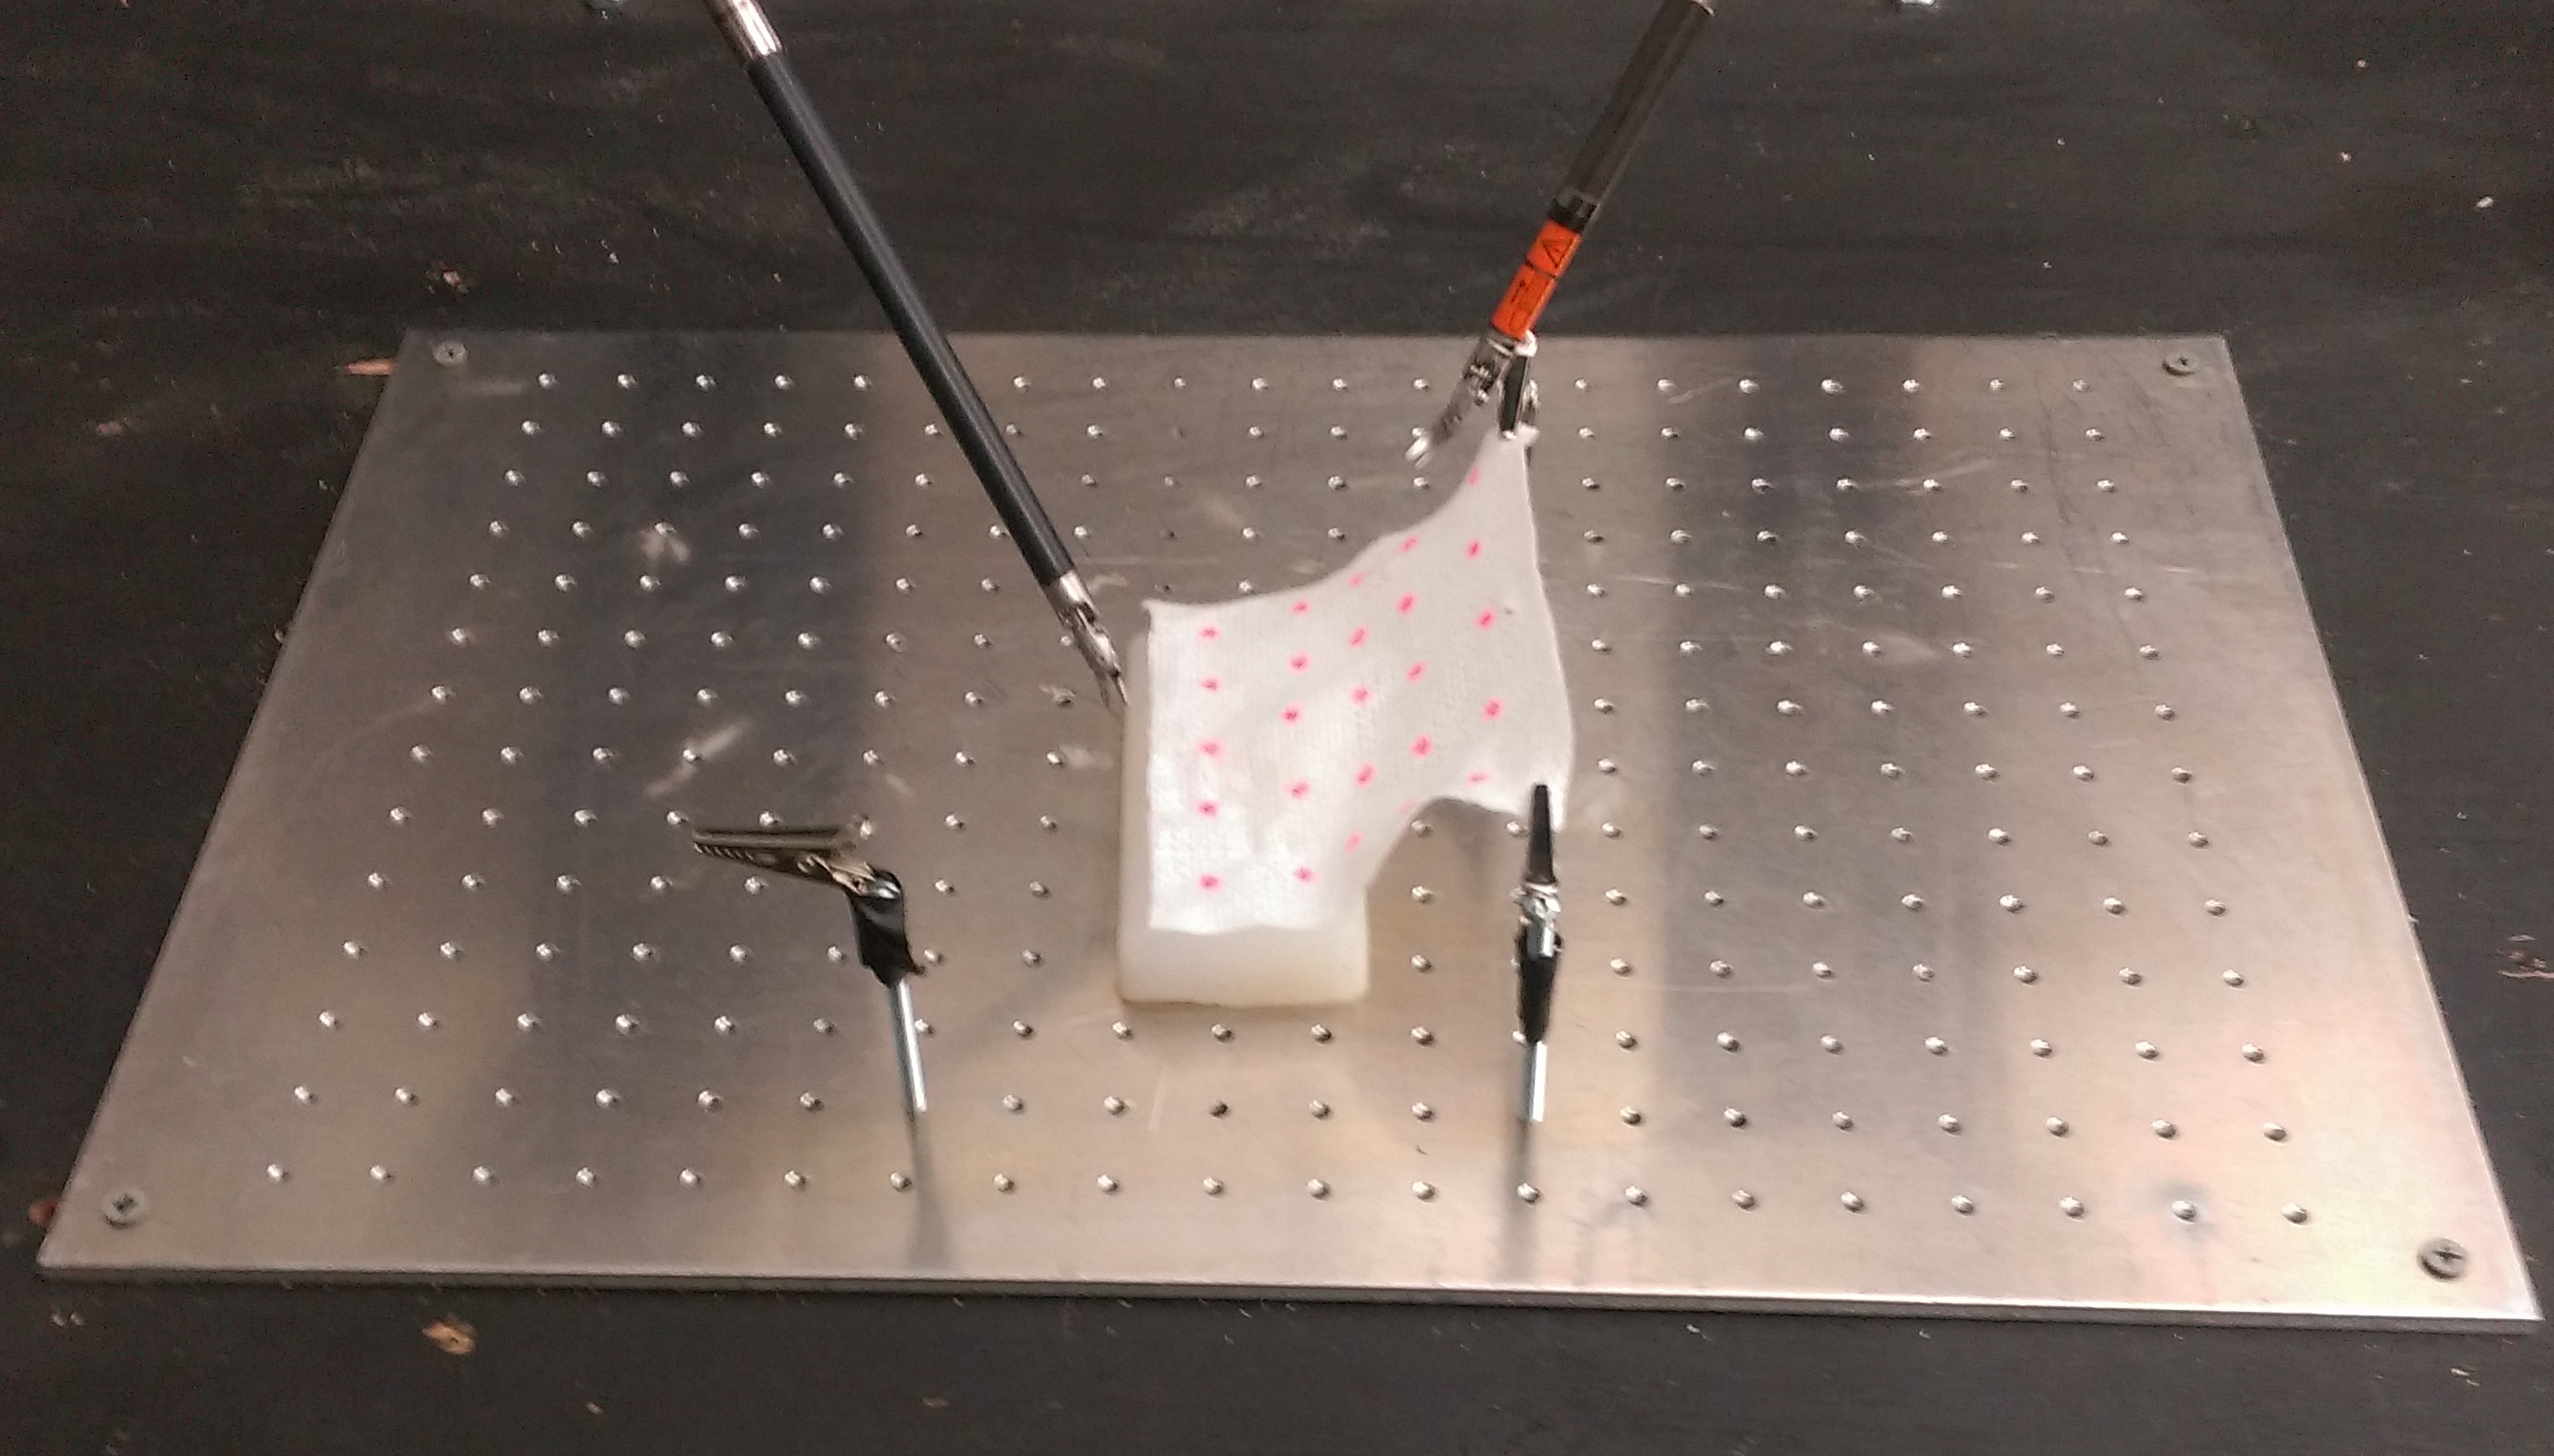
\includegraphics[width=0.8\columnwidth]{exp/IMAG0249.jpg}
    \caption{The experimental setup for gauze grasping and tensioning. The task is to grasp the gauze and lift it to flatten it out. This task is not usually successful in an open-loop trajectory due to deformation after the grasp.
    }
    \label{exp:dvrk2}
% \vspace{-15pt}
\end{figure}

\begin{figure}[t]

    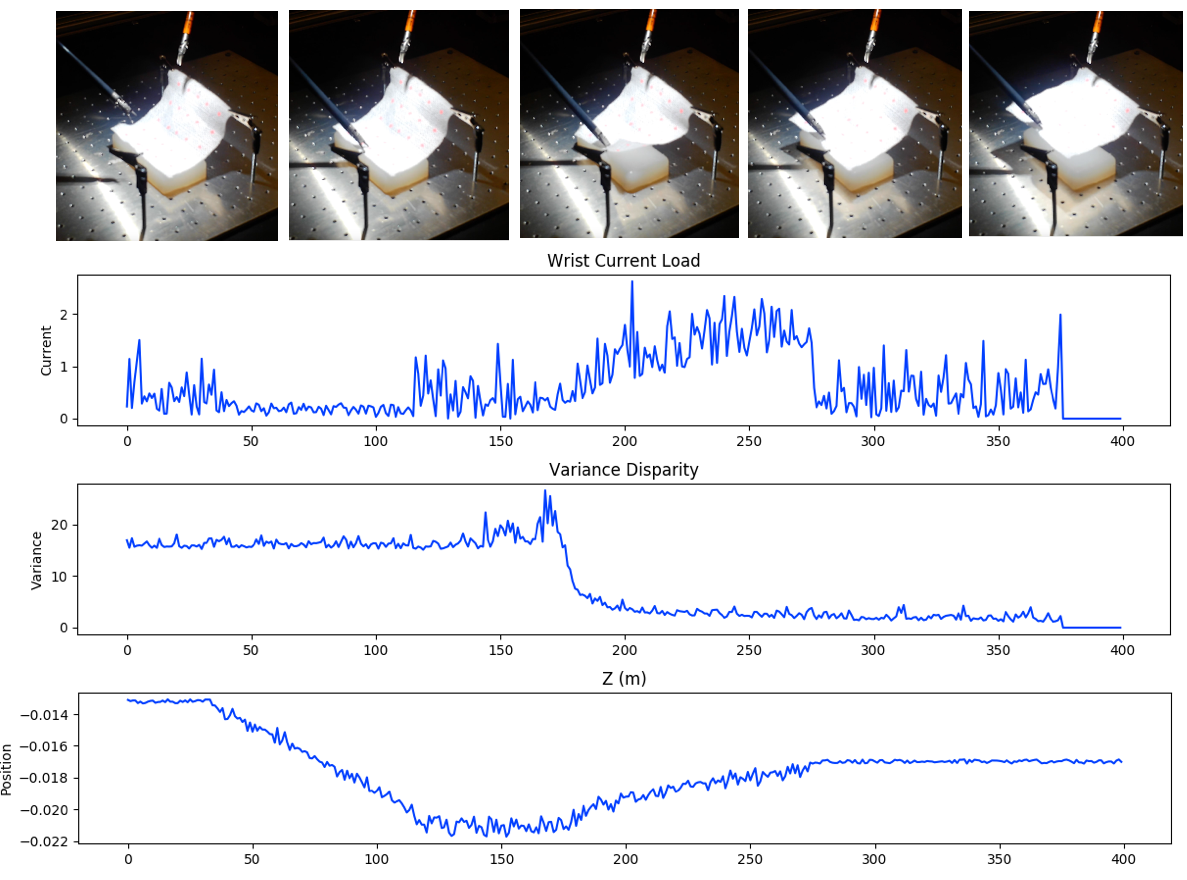
\includegraphics[width=\columnwidth]{exp/signals.png}
    \raggedright
    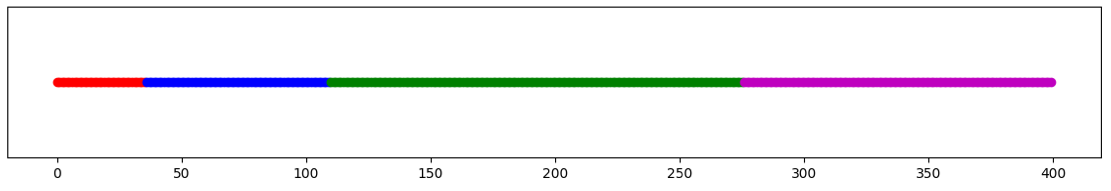
\includegraphics[width=0.9\columnwidth]{exp/segmentation.png}
    \caption{A representative demonstration of the deformable sheet grasping task with relevant features plotted over time. \hirl identifies 4 segments when applied to the deformable sheet grasping task. 
    }
    \label{exp:dvrk3}
% \vspace{-15pt}
\end{figure}

\subsubsection{Acrobot}\label{exp:acrobot}
This domain consists of a two-link pendulum with gravity and with torque controls on the joint. The dynamics are noisy and there are limits on the applied torque. The robot has 1000 timesteps to raise the arm above horizontal ($y=1$ in the images). If the task is successful and the robot receives a reward of $1$. 
Thus, the expected reward is equivalent to the probability that the current policy will successfully raise the arm above horizontal.
We generated $N=5$ demonstrations for the Acrobot task and applied segmentation. 
These demonstrations were generated by training the Q-Learning baseline to convergence and then sampling from the learned policy.
%We visualize the learned segments in Figure \ref{exp:acroseg}, which can be seen to qualitatively describe a successful path.
In Figure \ref{exp:acsegmentation-res2}, we plot the performance of the all of the approaches.
We include a comparison between a Linear Multiclass SVM and a Kernelized Multiclass SVM for the policy learning alternative.
In this example, we find that applying MaxEnt-IRL does not improve the convergence rate.
For this state-space, MaxEnt-IRL merely recovers the reward used in the original RL problem.
On the other hand, added segments using \hirl improve convergence rates.

% the \hirl approaches add segments making it easier to converge.

We also vary the number of input demonstrations to \hirl and find that it requires fewer demonstrations than policy learning and MaxEnt-IRL to converge to a more reliable policy.
It takes about 10x more demonstrations for the supervised learning approach to reach comparable reliability.
Finally, we find that \hirl does not sacrifice much transferability.
We learn the rewards on the standard pendulum, and then during learning we vary the size of the second link in the pendulum.
We plot the success rate (after a fixed 50000 steps) as a function of the increase link size.
\hirl is significantly more robust than supervised policy learning to the increase in link size and has a significantly higher success rate than IRL for small perturbations in link size. 

\subsection{Physical Experiments with the da Vinci Surgical Robot}


\subsubsection{Deformable Sheet Grasping and Tensioning: } Next, we apply \hirl to learn to how to grasp and tension a sheet of gauze. The experimental setup is pictured in Figure \ref{exp:dvrk2}. The basic setup is a sheet of gauze fixtured at the two far corners. The robot's task to the grasp the gauze on the opposing side, lift it up, and in the process flatten the sheet out.
This task is not usually successful in an open-loop trajectory due to deformation after the grasp.
Some grasps pick up more or less of the material and the flattening procedure has to be accordingly modified.
The state-space is the 6 DoF end-effector position of the robot, the current load on the wrist of the robot, and a visual feature measuring the differences in disparity markers on the sheet (a proxy for flatness).
The action space is discretized into an 8 dimensional vector ($\pm x$, $\pm y$, $\pm z$, open/close gripper) where the robot moves in 2mm increments.

We provided 15 demonstrations through a keyboard based tele-operation interface.
From these 15 demonstrations, \hirl identifies four segments. Figure \ref{exp:dvrk3} illustrates the segmentation of a representative demonstration with important states plotted over time.
In this problem, we applied both the model-based and model-free versions of \hirl to construct the rewards.
One of the segments corresponds to moving to the correct grasping position, one corresponds to making the grasp, one lifting the gauze up again, and one corresponds to straightening the gauze.

We can use the reward functions learned by \hirl to refine the policy for this task.
We define a Q-Network with a single-layer Multi-Layer Perceptron with 32 hidden units.
For each of the segments, we apply Behavioral Cloning locally with the same architecture as the Q-network (with an additional softmax over the output layer) to get an initial policy. We rollout 100 trials with an $\epsilon=0.1$ greedy version of these segmented policies.
The learning results of this experiment are summarized below with different variations of the learning algorithms.
The value of the policy is a measure of average disparity over the gauze accumulated over the task (if the gauze is flatter longer, then the value is greater).
As a baseline, we applied RL for 100 rollouts with no other information. RL did not successfully grasp the gauze even once.
Next, we applied behavioral cloning (BC) directly.
BC was only able to reach the gauze and distrub it but not succesfully grasping.
Then, we applied the segmentation from \hirl  and applied BC directly to each local segment (without further refinement). 
This was able complete the full task.
Finally, we applied all of \hirl and found the highest-value results.
For comparison, we applied \hirl without the BC initialization and found that it was only successful at the first two steps.

% Please add the following required packages to your document preamble:
% \usepackage[table,xcdraw]{xcolor}
% If you use beamer only pass "xcolor=table" option, i.e. \documentclass[xcolor=table]{beamer}
\begin{table}[]
\centering
\scriptsize
\caption{Results from the deformable sheet grasping experiment}
\label{my-label}
\begin{tabular}{llll}
\rowcolor[HTML]{000000} 
{\color[HTML]{FFFFFF} Technique} & {\color[HTML]{FFFFFF} \# Demonstrations} & {\color[HTML]{FFFFFF} \# Rollouts} & {\color[HTML]{FFFFFF} Value} \\
RL (ab initio)                   & -                                        & 100                                & -8210                        \\
BC                               & 15                                       & -                                  & -7591                        \\
Segmentation+BC                  & 15                                       & -                                  & -3516                        \\
SWIRL+MF (no init)                  & 15                                       & 100                                & -6128                        \\
SWIRL+MB (no init)                  & 15                                       & 100                                & -5798                        \\
\textbf{SWIRL+MF (BC init)}                  & 15                                       & 100                                & \textbf{-3110}     \\
\textbf{SWIRL+MB (BC init)}                  & 15                                       & 100                                & \textbf{-2241}                       
\end{tabular}
\end{table}

\subsubsection{Surgical Line Cutting: }
In the next experiment, we evaluate generalization to different task instances.
We apply \hirl to learn to cut along a marked line in gauze similar to Murali et al.~\cite{murali2015learning}.
This is a multi-step problem where the robot starts from a random initial state, has to move to a position that allows it to start the cut, and then cut along the marked line.
We provide the robot 5 kinesthetic demonstrations by positioning the end-effector and then following various marked straight lines.
The state-space of the robot included the end-effector position $(x,y)$ as well as a visual feature indicating its pixel distance to the marked line $(pix)$.
This visual feature is constructed using OpenCV thresholding for the black line.
Since the gauze is planar, the robot's actions are unit steps in the $\pm x, \pm y$ axes.
Figure\,\ref{exp:dvrk1} illustrates the training and test scenarios.

\hirl identifies two segments corresponding to the positioning step and the termination.
The learned reward function for the position step minimizes $x,y,pix$ distance to the starting point and for the cutting step the reward function is more heavily weighted to minimize the $pix$ distance.
We defined task success as positioning within $1$\,cm of the starting position of the line and during the following stage, missing the line by no more than $1$\,cm (estimated from pixel distance).
We evaluated the model-free version of \hirl, Q-Learning, and Behavioral Cloning with an SVM.
\hirl was the only technique able to achieve the combined task.
This is because the policy for this task is non-stationary, and \hirl is the only approach of the alternatives that can learn such a policy.

We evaluated the learned tracking policy to cut gauze.
We ran trials on different sequences of curves and straight lines. 
Out of the 15 trials, 11 were successful.
2 failed due to \hirl errors (tracking or position was imprecise) and 2 failed due to cutting errors (gauze deformed causing the task to fail).
1 of the failures was on the 4.5 cm curvature line and 3 were one the 3.5 cm curvature line.

% \begin{figure}[t]
% \centering
%  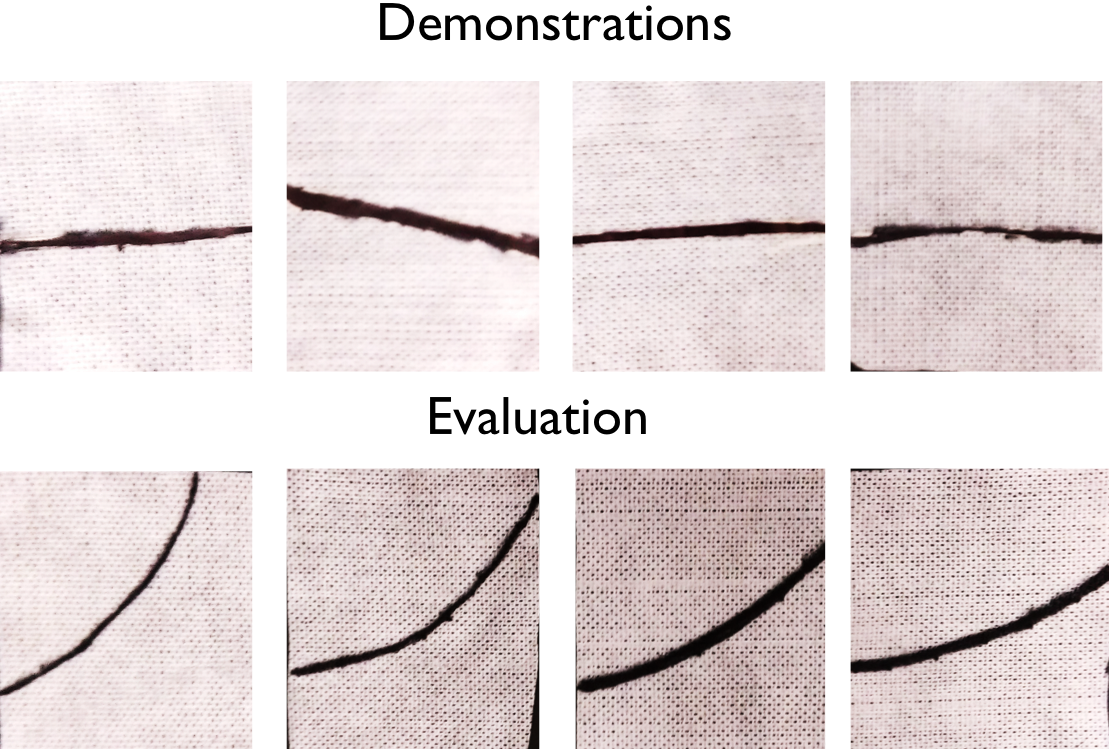
\includegraphics[width=0.7\textwidth]{exp/dvrk-demos-1.png}
%  \caption{We collected demonstrations on the da Vinci surgical robot kinesthetically. The task was to cut a marked line on gauze. We demonstrated the location of the line without actually cutting it. The goal is to infer that the demonstrator's reward function has two steps: position at a start position before the line, and then following the line. We applied this same reward to lines that were not straight nor started in exactly the same position.\label{exp:dvrk1}}
% \end{figure}

% \begin{SCfigure}[10][t]
%     \centering
%     \vspace{-0.5em}
%     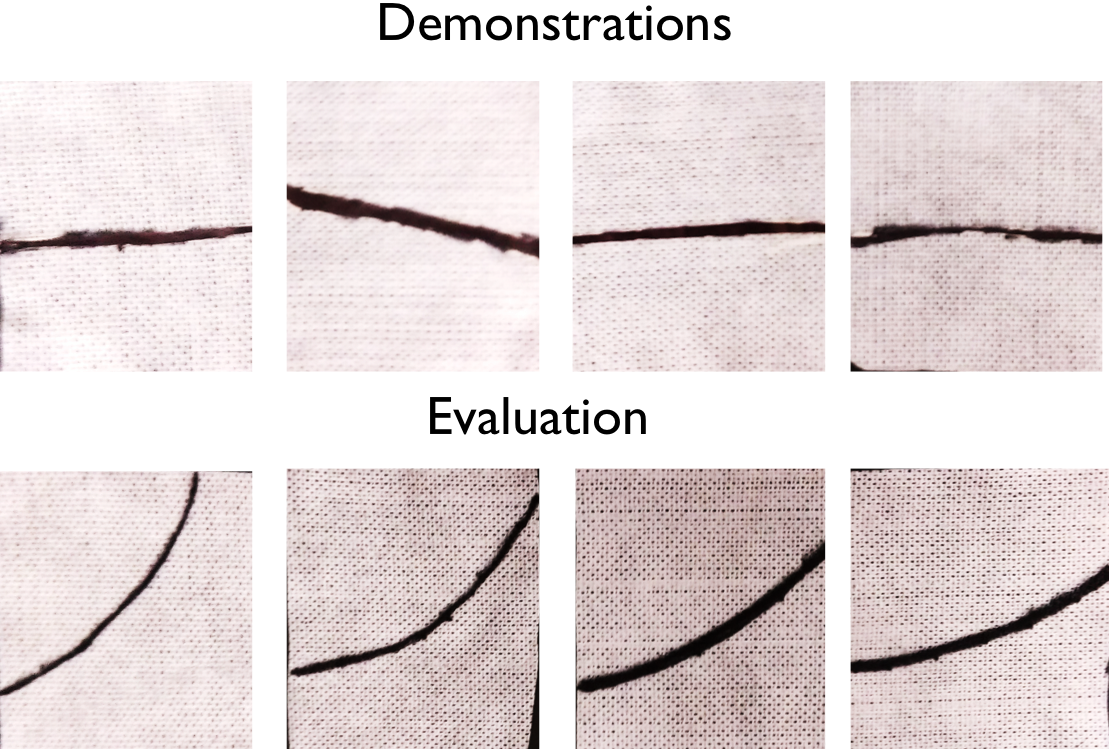
\includegraphics[width=0.5\textwidth]{exp/dvrk-demos-1.png}
%     \caption{We collected demonstrations on the da Vinci surgical robot kinesthetically. The task was to cut a marked line on gauze. We demonstrated the location of the line without actually cutting it. The goal is to infer that the demonstrator's reward function has two steps: position at a start position before the line, and then following the line. We applied this same reward to lines that were not straight nor started in exactly the same position.}
%     \label{exp:dvrk1}
%     \vspace{-1.5em}
% \end{SCfigure}


\begin{figure}[t]
\centering
    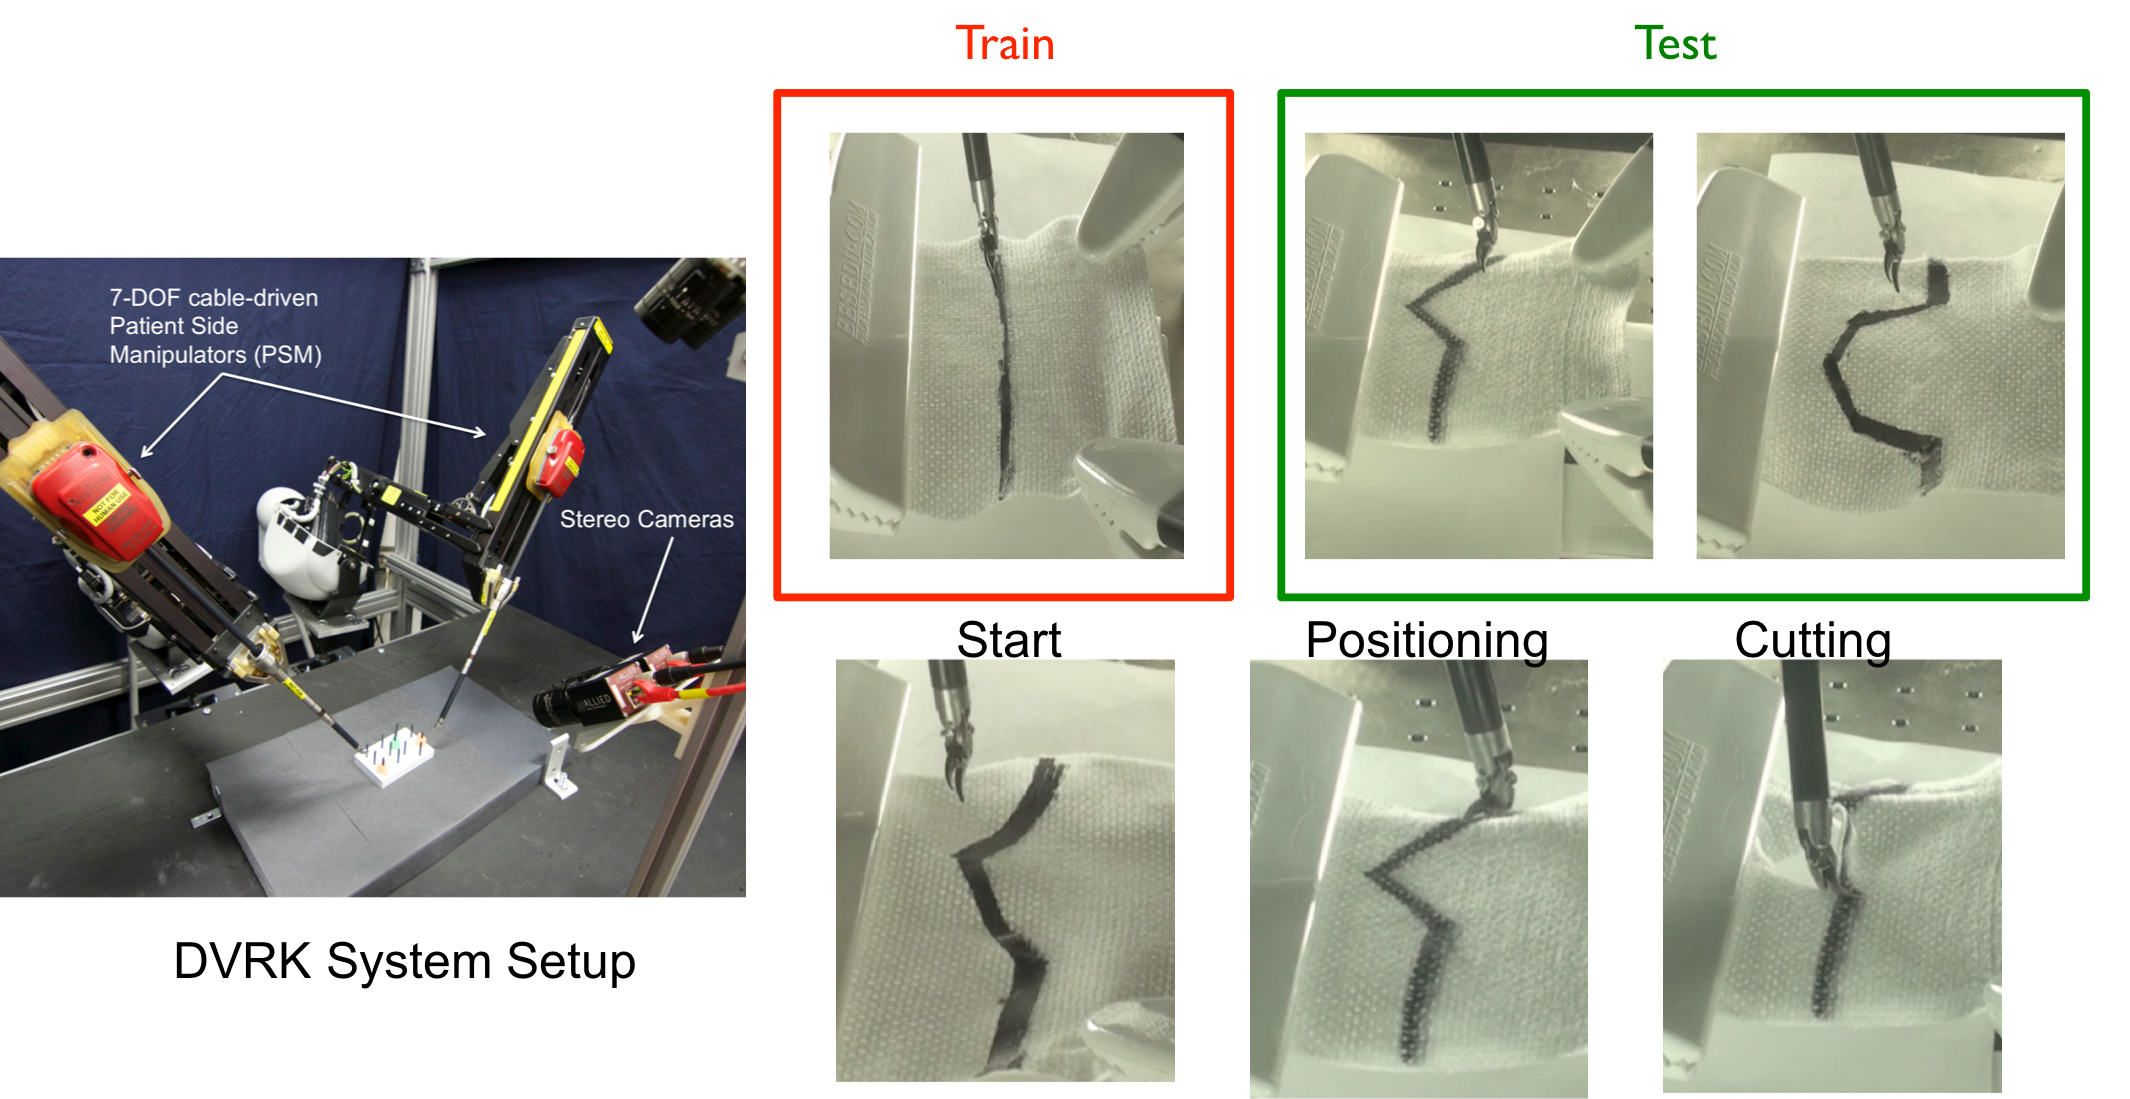
\includegraphics[width=\columnwidth]{exp/dvrk-demo-2.png}
    \caption{
      We collected demonstrations on the da Vinci surgical robot kinesthetically. The task was to cut a marked line on gauze. We demonstrated the location of the line without actually cutting it. The goal is to infer that the demonstrator's reward function has two steps: position at a start position before the line, and then following the line. We applied this same reward to curved lines that started in different positions.
    }
    \label{exp:dvrk1}
% \vspace{-15pt}
\end{figure}

\begin{table*}[ht]
    \centering
    \caption{With 5 kinesthetic demonstrations of following marked straight lines on gauze, we applied \hirl to learn to follow lines of various curvature. After 25 episodes of exploration, we evaluated the policies on the ability to position in the correct cutting location and track the line. We compare to SVM on each individual segment. SVM is comparably accurate on the straight line (training set) but does not generalize well to the curved lines.
    \label{dvrk:res1}}
    \resizebox{\linewidth}{!}{% put in textwidth
    \begin{tabular}{c||c|c|c|c}
    \hline
    \rowcolor[HTML]{CBCEFB} 
    Curvature Radius (cm) & SVM Pos. Error (cm) & SVM Tracking Error (cm) & \hirl Pos. Error (cm) & \hirl Tracking Error (cm) \\
     \hline \hline
    straight & 0.46 & 0.23 & 0.42 & 0.21  \\
    \rowcolor[HTML]{E0E0E0} 
    4.0 & 0.43 & 0.59 & 0.45 & 0.33 \\
    3.5 & 0.51 & {\color{red}\textbf{1.21}} & 0.56 & 0.38 \\
    \rowcolor[HTML]{E0E0E0} 
    3.0 & 0.86 & {\color{red}\textbf{3.03}} & 0.66 & 0.57 \\
    2.5 & {\color{red}\textbf{1.43}} & {\color{red}-} & 0.74 & 0.87 \\
    \rowcolor[HTML]{E0E0E0} 
    2.0 & {\color{red}}- & {\color{red}}- & 0.87 & {\color{red}\textbf{1.45}} \\
    1.5 & {\color{red}}- & {\color{red}}- & {\color{red}\textbf{1.12}} & {\color{red}\textbf{2.44}} \\
     \hline
    \end{tabular}
    }
    % \vspace{-10pt}
\end{table*}

Next, we characterized the repeatability of the learned policy.
We applied \hirl to lines of various curvature spanning from straight lines to a curvature radius of 1.5 cm.
Table \ref{dvrk:res1} summarizes the results on lines of various curvature.
While the SVM approach did not work on the combined task, we evaluated its accuracy on each individual step to illustrate the benefits of \hirl.
On following straight lines, SVM was comparable to \hirl in terms of accuracy.
However, as the lines become increasingly curved, \hirl generalizes more robustly than the SVM.


